\section{Docker image}
\label{sec:intro:docker_image:docker_img}
This section explains the Docker image in more detail. First the architecture of a Docker image with the most necessary information for subsequent work is presented. Then the construct for building a Docker image is explained. 
Lastly a description of the metadata information of an image takes place. These basics are very important as they are part in the theoretical concept.

\subsection{Image architecture}
\label{sec:intro:docker_image:docker_img:architecture}
A Docker image is ultimately a stack of selected file system layers to provide a starting point for a container.
Figure \ref{sec:intro:docker_image:docker_image_stack} shows how a Docker image is stacked. At the bottom there is the Linux kernel. A Debian and a Busybox are placed on the kernel.
Both of them are runnable base images.
On top of these layers can be more layers stacked as shown on the Debian layer with an additional Emacs and an Apache layer. The busybox itself does not have another further layer placed on the top.
Docker finally attaches a read/write file system across all underlying layers when a container is launched from an image. This can be seen on both images in this example.

\begin{figure}[htbp]
 \centering
 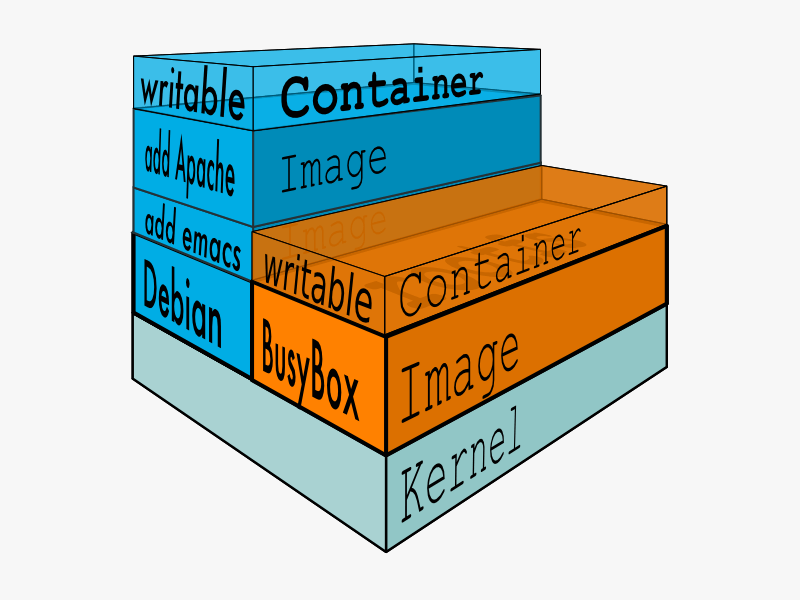
\includegraphics[width=0.6\textwidth]{gfx/examples/docker-filesystems-busyboxrw}
 \caption{Docker filesystems stacked to represent an image}
\label{sec:intro:docker_image:docker_image_stack}
\end{figure}
Docker uses storage drivers in order to manage images and especially corresponding file system layers. Each storage driver handles the implementation differently.
There are several storage drivers available like ZFS, BTRFS and many more which can be configured by the responsible system-engineer or developer. Docker uses in the latest version Overlay2 as storage driver per default. The Overlay2 informations about an image can be viewed by the Docker inspect command.
\begin{lstlisting}
	docker inspect ubuntu
\end{lstlisting}
In order to show only the part of interest for the docker image architecture, the inspection delivers a tailored result.
\lstinputlisting[caption={Docker inspection results}, firstline=71, lastline=79, captionpos=b, label={sec:intro:docker_image:corresponding_unionfs}]{chapters/intro/listings/inspect_results.txt}

As seen in Listing \ref{sec:intro:docker_image:corresponding_unionfs} the introduced mechanisms of the Overlay2 union file system \ref{sec:intro:docker_image:unionfs} are completely used.
This shows once again that Docker only uses the well-known core functions of Linux instead of building its own mechanisms.
One interesting and important fact is the mount process. The lower-directories are not mounted directly by their folder name. Docker uses for each image layer a symbol link. The reason is only the total length of 65 characters for each folder name. These symbolic links help avoid the Linux ‘mount’ command from exceeding page size limitation.
Also it is important to note that the \textbf{diff} directory in each layer builds the chain of the overlay. In each layer are additional helper files available like the lowerfile which creates a relation to associated parent. This lowerfile exists only if a parent folder exist.
The lower files are responsible for creating the correct order from the most upper layer to the lower layers.

Furthermore every image has a name and a tag. An image name is made up of slash-separated name components, optionally prefixed by a registry hostname. The hostname must comply with standard DNS rules, but may not contain underscores. A tag name must be valid ASCII and may contain lowercase and uppercase letters, digits, underscores, periods and dashes. A tag name may not start with a period or a dash and may contain a maximum of 128 characters.
It is important to know that the name and the tag are separated by a colon.
This knowledge about the naming and tagging connection is helpful, since it finds application in the following chapters. In the following the construct of building a Docker image called Dockerfile is described.

\subsection{Dockerfile}
\label{sec:intro:docker_image:docker_img:dockerfile}
In order to build a Docker image Docker Inc. introduced a construct called Dockerfile.
Each entry in this Dockerfile starts with a keyword. These keywords can be used by a developer to assemble an image. Each entry in a Dockerfile creates a different file system layer. In other words each file system layer represents an instruction with help of a keyword in a Dockerfile.
The Dockerfile construct provides around 20 keywords \cite{dockerfile_ref}.
Listing \ref{sec:intro:docker_image:dockerfile} shows a typical Dockerfile.
\lstinputlisting[caption={Dockerfile}, captionpos=b, label=sec:intro:docker_image:dockerfile]{chapters/intro/listings/dockerfile.txt}
The FROM statement starts out by creating a layer from the ubuntu:18.04 image. The COPY command adds an example bash script from the Docker client’s current directory. The RUN command makes the program executable. Finally the last layer specifies which command has to be executed inside the container.

An image can be created with the corresponding Dockerfile and the command Docker build. The responsible Docker command is shown below.
\begin{lstlisting}
	docker build <my_new_image> -f <dockerfile>
\end{lstlisting}
The Dockerfile construct is valuable to know because it is responsible for integrating secrets into an image. 
Logically there are two categories in a Dockerfile that contain commands that are responsible for integrating static files.
First \textit{direct integration} which is related the actions COPY and ADD. The difference between the two commands is the range of functions. Instead of COPY, ADD is able to unzip an archive directly to the endpoint.
Also ADD can request files, folders and archives from an URL and save the content directly to the endpoint.

The second category \textit{indirect integration} is a bit more comprehensive. This category is formed solely by the action RUN.
Docker itself uses RUN to trigger a shell command and commit it to a new image layer.
The executed shell commands for RUN are inline defined. That allows cases, loop-constructs and external program execution. A flexible bunch of code is allowed since it is just standard bash. This allows a developer to use available tools like ssh-keygen, openssl and manual file and folder creation. It is totally up to the developer what do to with that inline command in the Dockerfile. 

At this time it is known what a Docker image is and how it can be built. Also it is known to integrate static files into an image in an indirect and direct way. The next subsection introduces the important topic of the metadata of an image.

\subsection{Image metadata}
\label{sec:intro:docker_image:docker_img:meta}
Another important part is the metadata of an image. Every Docker image saves informations of the build process locally on a system.  
These informations are locally provided and accessible for the root user. 
In this work it is assumed hat no manipulation of the metadata was performed locally. 

The metadata is accessible through the Docker history command. The output of an Ubuntu 18.04 is shown below in Listing \ref{sec:intro:docker_image:meta}:
\lstinputlisting[caption={Prototype structure in Python}, captionpos=b, label={sec:intro:docker_image:meta}]{chapters/main/practical/listings/meta.txt}
On one hand this listing might be confusing. On the other hand it is helpful to get an overview how the meta data is structured.
Through the help of the history command the data is representated similar to JSON. The only difference is that numeral values are not marked in quotations. In this structure there are many attributes with their corresponding values. Attributes like "Created", "CreatyBy" are first followed by "Id" and many more. 	
Important informations are most of all Dockerfile instructions like COPY, ADD an RUN since they are responsible for integrating static files into the image.
In this example it can be seen that only an ADD command as Dockerfile keyword is used. A COPY method is not used.
A special fact applies to the RUN command. RUN commands are not directly listed in the meta informations.
Instead only the executable command that follows a RUN command is visible.

The analyzing of these informations is with the help of the history command easily done.
This is due to the javascript object notation similarity.
The metadata of Docker images provides a lot of information about a Docker image even if the Docker file is not available. Important properties can be extracted, such as Dockerfile keywords and corresponding parameters.
Also used RUN commands are included in the information by representations.

This chapter provided a basic knowledge about the architecture of Docker images and the interaction with Overlay2. To get an idea how the file structure is working behind the scenes this knowledge is fundamental. There are essential suggestions for the theoretical concept, which methods exist to integrate secrets into an image.
Before a theoretical concept is developed related work is shown about key leak techniques. Key leak techniques are essential in order to detect secrets.